\chapter{Theory}

\section{Gamma-ray Spectroscopy}

In this section, the physics responsible for the features in gamma-ray spectra are described. Also described are factors that complicate gamma-ray spectroscopy, including changing background radiation fields and temperature effects on detector calibration.

\subsection{Energy Deposition Mechanisms}

When a photon interacts with some radiation detection medium, it deposits some or all of it's energy into the material. There are three main methods of interaction: the photoelectric effect, Compton scattering, and pair production. These effects are energy dependent, as seen in Figure \ref{fig:energy_dependence_interactions}.

If the total of the photon's energy is deposited in the detector, a count is recorded in the spectrum's photopeak. If the photon deposits only a part of it's energy and escapes the detector, a count will be recorded somewhere below the full-energy photopeak.  The following sections describe intrinsic mechanisms that remove counts from the full-energy peak.% Absolute efficiency is also affected by shielding material and source-to-detector distance.

\subsubsection{Photoelectric effect}

The photoelectric effect occurs when a photon is absorbed by an atom in some material. This absorption produces a photoelectron, which has the energy of the photon minus the binding energy of the electron. The photoelectron is typically absorbed by the material, resulting in full-energy deposition. This process also creates a vacancy in the atom of the material. This vacancy is filled by another electron in the material, releasing a characteristic x-ray or Auger electron. Because of their low energies, Auger electrons are typically quickly reabsorbed. The characteristic x-ray can either be reabsorbed by the material or escape.

\begin{figure}[H]
\centering
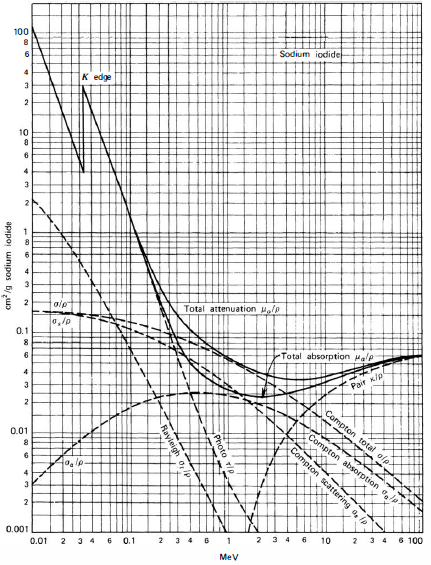
\includegraphics[width=0.75\linewidth]{images/energy_dependence_interactions}
\caption{Energy dependence for gamma-ray interactions in NaI \cite{knoll}.}
\label{fig:energy_dependence_interactions}
\end{figure}

\subsubsection{Compton scattering}

Compton scattering and absorption is the interaction of a gamma-ray photon with an electron in some absorbing material. This interaction is illustrated in Figure \ref{fig:compton_scatter}. 


% This is the main energy deposition mechanism in the range of energies useful for gamma-ray spectroscopy.

\begin{figure}[H]
\centering
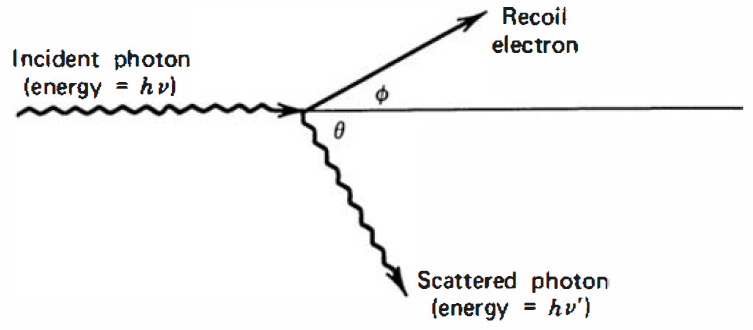
\includegraphics[width=0.8\linewidth]{images/compton_scatter}
\caption{Diagram of a Compton scattering event \cite{knoll}.}
\label{fig:compton_scatter}
\end{figure}

The energy of a photon scattered off a free electron

\begin{equation} \label{eq:compton_scatter}
E' = \frac{E}{1 + \frac{E}{m_{0} c^2} (1-cos\theta)}
\end{equation}

depends on the scattering angle, $\theta$, and the incident photon's energy, E. In equation \ref{eq:compton_scatter} m$_{0}$c$^{2}$ is the rest mass of the electron. A photon scattering at an angle of 180$^{o}$ deposits it's maximum amount of energy into a medium. Photons that escape after this energy deposition create the Compton edge observed in Figure \ref{fig:ideal_compton}. Photons that escape the detector after single or multiple Compton scatter events at angles less than 180$^{o}$ create the continuum of energies also seen in Figure \ref{fig:ideal_compton}. Accounting for the binding energy of electrons in a medium produces a Compton continuum closer to the dotted line in Figure \ref{fig:ideal_compton}.

\begin{figure}[H]
\centering
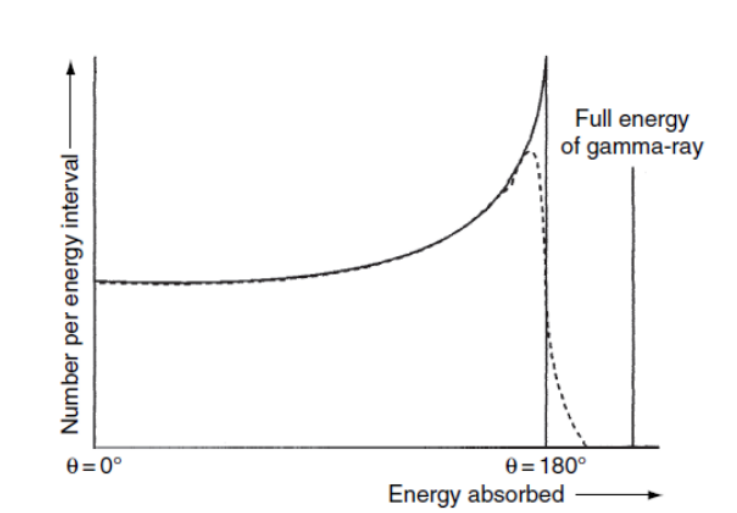
\includegraphics[width=0.75\linewidth]{images/ideal_compton}
\caption{Diagram of an idealized Compton scattering event \cite{gilmore}.}
\label{fig:ideal_compton}
\end{figure}



\subsubsection{Pair Production}

When a photon with energy above 1022 keV interacts with the coulomb field of a nucleus, there is a probability that the photon will disappear and be replaced by an electron-positron pair. The positron will then annihilate with an electron in the medium, creating two 511 keV photons. This process is illustrated in Figure \ref{fig:pair_production}. Because one or both of these annihilation photons can escape the detector, they can produce single or double escape peaks in a gamma-ray spectrum. As seen in Figure \ref{fig:pair_production_spectra}, single escape peaks occur at 511 keV below the full-energy peak and double escape peaks occur at 1022 keV below this peak. These 511 keV photons may also be measured by the detector, producing an annihilation radiation signal in the spectrum.

\begin{figure}[H]
\centering
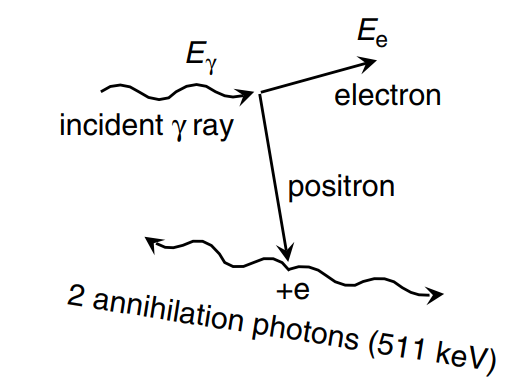
\includegraphics[width=0.6\linewidth]{images/pair_production}
\caption{Diagram of pair production \cite{gilmore}.}
\label{fig:pair_production}
\end{figure}

\begin{figure}[H]
\centering
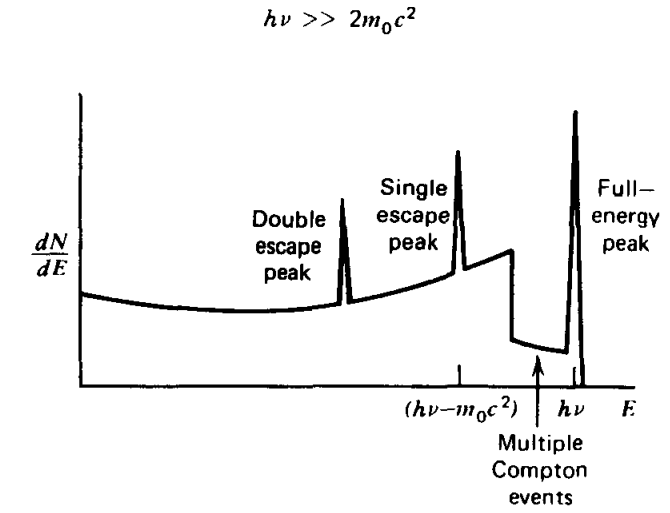
\includegraphics[width=0.6\linewidth]{images/pair_production_spectra}
\caption{Theoretical spectrum from pair production \cite{knoll}.}
\label{fig:pair_production_spectra}
\end{figure}


\subsection{Energy Resolution}

The energy resolution of a radiation detector describes how broad a photopeak is in a detector's spectrum. The resolution is based on the full width of the Gaussian at half of it's maximum value (FWHM). The FWHM is measured either in units of energy or as a percent of the peaks energy. This broadening is mostly due to statistical fluctuations in the number of information carriers produced in the detection system. Other factors that increase the resolution in scintillation detectors include nonproportionality of light yield per energy absorbed, the variance in photoelectron collection in the photocathode, and the variance in electrons produced in the photomultiplier tube \cite{knoll}. Because semiconductor detectors more directly measure charge carriers, they do not suffer the resolution losses associated with transforming information carriers. In addition to this, the variance in information carriers produced for a given energy does not follow a Poisson process in semiconductor detectors. This effect is known as the Fano factor and it significantly decreases the resolution of semiconductor detectors below the theoretical Poisson limit. Because the resolution changes as function of energy, the resolution of a 662 keV photon from $^{137}$Cs is used as the standard of comparison. The energy resolution of three scintillator (NaI(Tl), LaBr, CeBr) and two semiconductor (CZT, HPGe) radiation detectors are seen in Table \ref{table:detector_resolutions}. Figure \ref{fig:Ba133_spectrum_different_detector_materials_Market_Survey_Report} compares a $^{133}$Ba spectrum from scintillation and semiconductor detectors. 

% pg 345 knoll

\begin{table}[H]
\centering
\begin{tabular}{|c|c|}
\hline
Detector Type & \begin{tabular}[c]{@{}c@{}}Full Width at Half Maximum\\ (662 keV)\end{tabular} \\ \hline
NaI(Tl) & 6 - 8 \% \\ \hline
LaBr & 2 - 4 \% \\ \hline
CeBr & 4 - 5 \% \\ \hline
CZT & 1 - 2 \% \\ \hline
HPGe & \textless 0.2 \% \\ \hline
\end{tabular}
\caption{Typical energy resolutions of different
gamma-ray detector types (reproduced from \cite{RIIDMarketSurveyReport}).}
\label{table:detector_resolutions}
\end{table}


\begin{figure}[H]
\centering
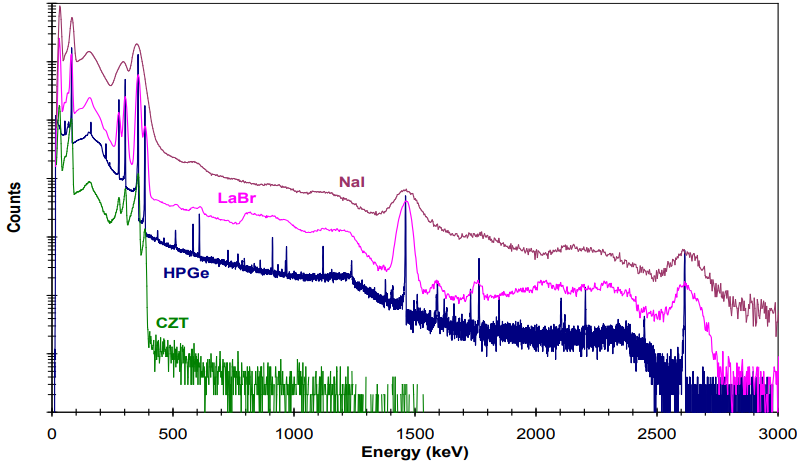
\includegraphics[width=0.8\linewidth]{images/Ba133_spectrum_different_detector_materials_Market_Survey_Report}
\caption{Ba133 spectrum measured using different detector materials \cite{RIIDMarketSurveyReport}.}
\label{fig:Ba133_spectrum_different_detector_materials_Market_Survey_Report}
\end{figure}


\subsection{Background Radiation}

A significant challenge to automated gamma-ray spectroscopy is the stochastic nature of the background radiation field. Background radiation comes from radioisotopes naturally distributed in the soil and cosmic radiation. Isotopes in the soil come from the uranium decay series, thorium  decay series, and $^{40}$K. The gamma-ray spectra from each of these sources are shown in Figure \ref{fig:background_components}. 

\begin{figure}[H]
\centering
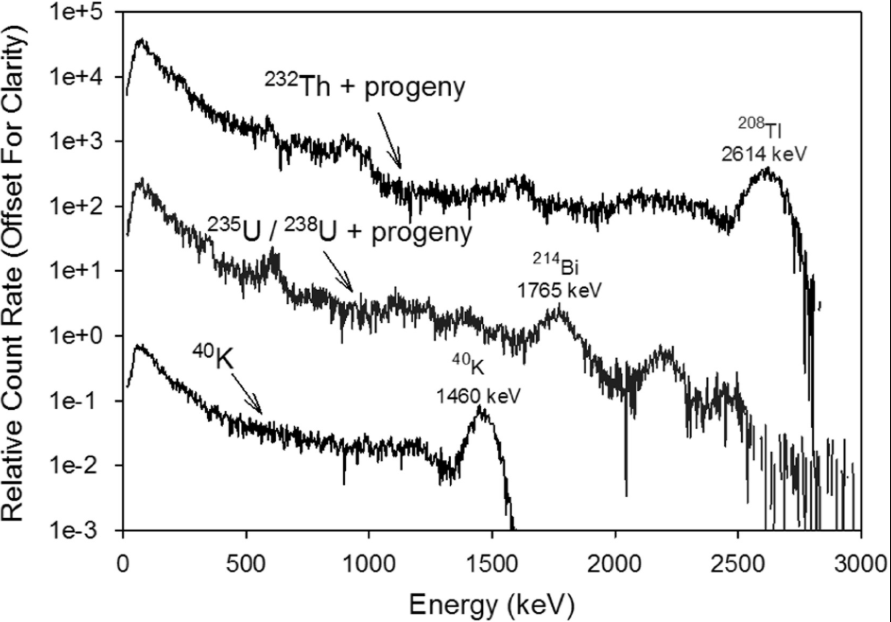
\includegraphics[width=0.8\linewidth]{images/background_components}
\caption{Monte Carlo simulations of background component spectra in NaI \cite{KULISEK2015}.}
\label{fig:background_components}
\end{figure}

These radiation components can change both spatially and temporally. Background radiation isotopes change geologically, (Figures \ref{fig:USGS_u_conc}, \ref{fig:USGS_th_conc}, and \ref{fig:USGS_k_conc}) creating different background radiation patterns in different parts of the country. Local changes in soil composition may also be significant enough to be observed in gamma-ray spectra. Because common building materials like concrete and granite contain radioactive elements, the proximity to structures can cause local variations in background. 

Background also changes over time. This change is largely due to the decay products of $^{222}$Rn gas generated by uranium decay in soil \cite{knoll}. Rain can also increase the level of background radiation by releasing trapped radon gas and other radioactive sources in the soil.

% Air Survey on Background Gradients https://www-sciencedirect-com.proxy2.library.illinois.edu/science/article/pii/S0265931X13002373

\begin{figure}[H]
\centering
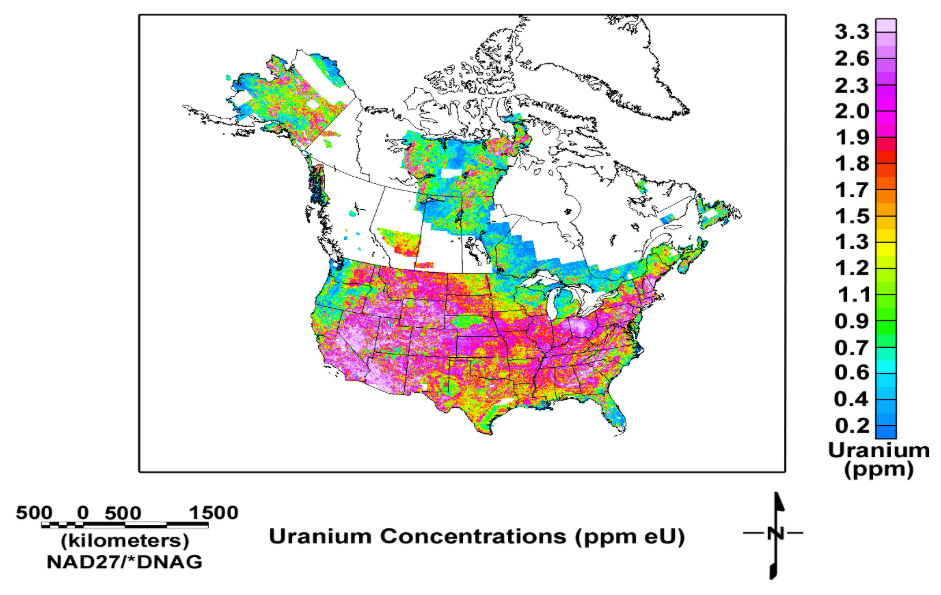
\includegraphics[width=0.9\linewidth]{images/USGS_u_conc}
\caption{Map of uranium concentrations in the United States \cite{USGS}.}
\label{fig:USGS_u_conc}
\end{figure}

\begin{figure}[H]
\centering
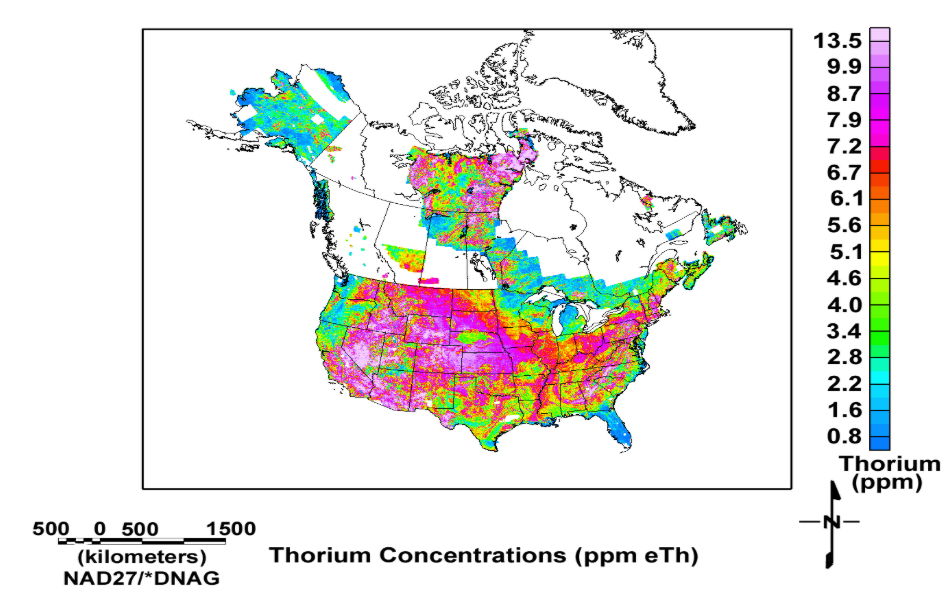
\includegraphics[width=0.9\linewidth]{images/USGS_th_conc}
\caption{Map of thorium concentrations in the United States \cite{USGS}.}
\label{fig:USGS_th_conc}
\end{figure}

\begin{figure}[H]
\centering
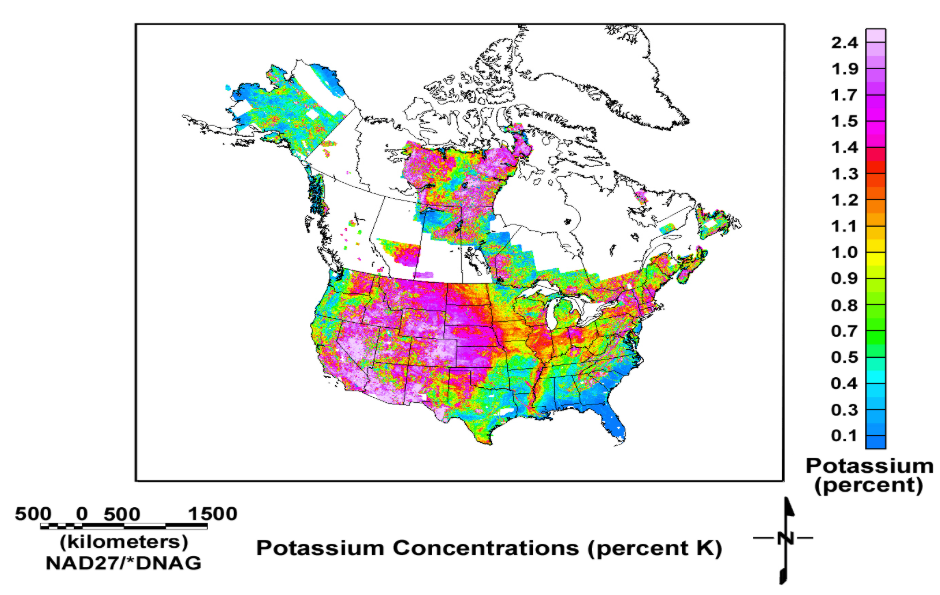
\includegraphics[width=0.9\linewidth]{images/USGS_k_conc}
\caption{Map of $^{40}$K concentrations in the United States \cite{USGS}.}
\label{fig:USGS_k_conc}
\end{figure}

% \USGS Open-File Report 2005-1413: Terrestrial Radioactivity and
%Gamma-ray Exposure in the United States and Canada," 2013.
% [Online]. Available: http://pubs.usgs.gov/of/2005/1413/maps.htm


\subsection{Affect of Temperature Change on Calibration}


Figure \ref{fig:CASANOVAS2012588} shows how relative peak position shifts with respect to changes in temperature of an ORTEC Model 905-3 2x2 NaI detector. Gain stabilization methods exist, but because they rely on clear photopeaks in a spectrum. they are not 

\begin{figure}[H]
\centering
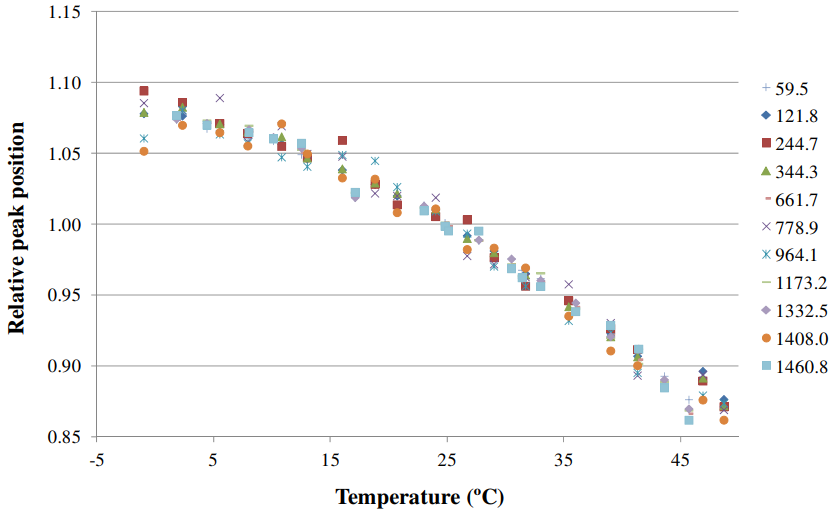
\includegraphics[width=0.95\linewidth]{images/temp_vs_relative_peak_position_CASANOVAS2012588}
\caption{Temperature vs relative photopeak position for an ORTEC Model 905-3 2x2 NaI detector \cite{CASANOVAS2012588}.}
\label{fig:CASANOVAS2012588}
\end{figure}




\section{Machine Learning}

In this section, neural network architectures and parameters that effect training will be described. Neural network architectures will include DNN, CNN, and the autoencoder. 

\subsection{Neural Network Architecture}

% Node/neruon, get this lingo straight here
An ANN is a mathematical model that attempts to map an arbitrary function from $\mathbb{R}^M$ to $\mathbb{R}^N$, where $M$ and $N$ are positive integers. An ANN accomplishes this by mimicking biological neurons. One example of an ANN architecture is shown in Figure \ref{fig:Network}. This ANN has N neurons in input layer A, J neurons in hidden layer B, and K neurons in output layer C. Each neuron in adjacent layers are connected by weights, represented in Figure \ref{fig:Network} by arrows connecting neurons. 


\begin{figure}[H]
\centering
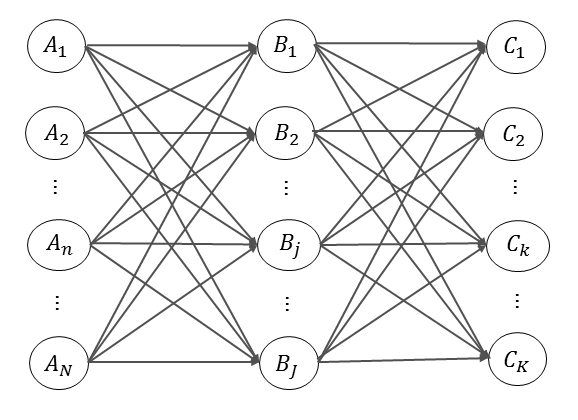
\includegraphics[width=0.75\linewidth]{images/Network}
\caption{Example ANN with input neurons $A_n$, hidden neurons $B_j$, and output neurons $C_k$.}
\label{fig:Network}
\end{figure}


Similar to a biological neuron, the ANN neuron receives input stimuli, performs an operation using it, and outputs the resulting signal. The structure and equation governing the operation of an individual neuron is shown in Figure \ref{fig:Node}. 

\begin{figure}[H]
	\centering
	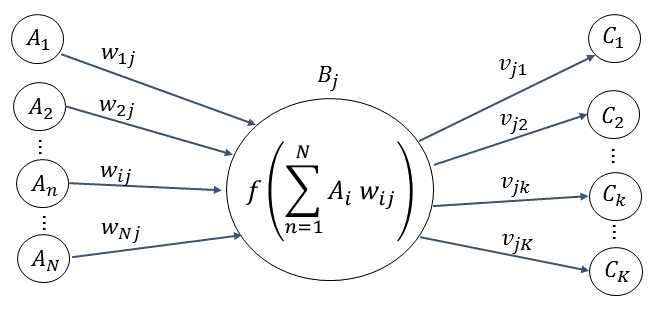
\includegraphics[width=0.75\linewidth]{images/Node_ABC_2}
	\caption{Summary of the operation of a single neuron.}
	\label{fig:Node}
\end{figure}

As seen in Figure \ref{fig:Node}, each neuron operates by summing the products of the previous layers values ($A_1$, $A_2$, ... $A_N$}) and each individual weight ($w_{1j}$, $w_{2j}$, ... $w_{nj}$) connecting the neurons. This summation is analogous to the stimulus a biologic neuron receives from its dendrites. The stimulus is then operated on by an activation function $f$, typically a non-linear function. The output signal is then passed to the next layer of the ANN where the process repeats. An ANN may be trained by setting the network weights, $\mathbf{W}$, in such a way that they minimize the error between target values, $\mathbf{T}$, in a training dataset, $\mathbf{Y}$, and the ANN output given that training dataset, $f( \mathbf{Y} ; \mathbf{W} )$, 
%
\begin{equation} \label{eq:argminW_Error}
\underset{\mathbf{W}}{\text{argmin}} {\text{ Error}}(f(\mathbf{Y} ; \mathbf{W} ) , \mathbf{T} ).
\end{equation}
% \underset{w}{\text{argmin}} \sum_{i=1}^{N} \Vert t_i - y_i \Vert^2
Except under simple cases, Equation \ref{eq:argminW_Error} cannot be solved analytically. Numerical methods for solving this equation include gradient descent through the back-propagation of errors \cite{Rumelhart1986}, genetic learning algorithms \cite{Yao1999}, and Newtons method \cite{Fletcher2000}.


\subsection{Simple Neural Network Example}

An example of a very simple one-layer ANN is shown in Figure \ref{fig:one_layer_net}. This ANN takes two inputs ($x_1$ and $x_2$) and performs the operation shown in Figure \ref{fig:Node}. The weights in the hidden layer connecting the $i^{th}$ input neuron to the $j^{th}$ output neuron will be represented by $w_{ij}$. The bias is set to a constant value of 1. This allows the bias to be effectively trained by changing the weights connecting the bias to the next layer. Using the hyperbolic tangent function, the network outputs for each class $y_1$, $y_2$, and $y_3$ range from -1 to 1. Using these outputs, any input can be classified into a given class if the class' respective output neurons value is above zero, or not in a class if the output neurons value is below zero. The equation for the output of the $j^{th}$ output is given in Equation \ref{eq:single_layer_eq_sum}, where $x_i$ is the $i^{th}$ input from the previous layer, and $b_i$ is the value of the weight connecting the $j^{th}$ output to the bias neuron.
%
\begin{equation} \label{eq:single_layer_eq_sum}
y_j = \tanh(\sum_i x_i w_{ij} + b_j),
\end{equation}

To more clearly understand the geometry of the network's operation, consider the dataset in Figure \ref{fig:training_set_one_layer}. This dataset is composed of three classes: red, green, and blue. The axes that define this dataset are the inputs to the single layer network in Figure \ref{fig:one_layer_net}, ($x_1$,$x_2$). If $\mathbf{W}$ is defined to be a vector with elements ($w_{11}$, $w_{21}$), a line can be defined perpendicular to $\mathbf{W}$ and shifted by $\frac{b_1}{||\mathbf{W}||}$ away from the origin in the direction of $\mathbf{W}$. Given appropriate values for $w_{11}$, $w_{21}$, and $b_1$, a line that separates the blue class from the non-blue class can be created. Any point on the -$\mathbf{W}$ side of the line will have $y_1 < 0$, allowing for classification. Similarly, a separating line for the red class using $w_{12}$, $w_{22}$, and $b_2$ and a separating line for the green class using $w_{13}$, $w_{23}$, and $b_3$ can be constructed. 

The classes in this example dataset are linearly separable, meaning lines can be drawn completely separating each class. If the classes were not linearly separable, additional hidden layers would be necessary to compute the function. It has been shown that additional hidden layers allow the creation of arbitrary decision boundaries \cite{Hornik1991}. 
%
\begin{figure}[H]
	\centering
	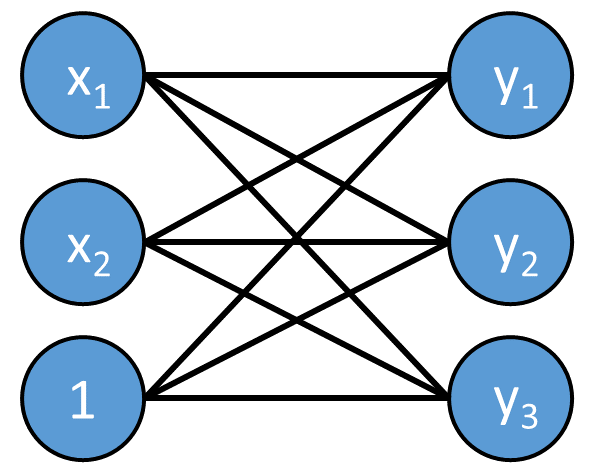
\includegraphics[width=0.45\linewidth]{images/One_layer_net_v31}
	\caption{Example of a single-layer neural network with two inputs ($x_{1}$ and $x_{2}$), three classes ($y_{1}$, $y_{2}$, $y_{3}$), and a bias neuron set to one.}
	\label{fig:one_layer_net}
\end{figure}
% Change these to diff objects to get around grey-scale thesis...?
%The neural network described in Figure \ref{fig:one_layer_net} has two inputs, so its decision boundaries are lines. If the network had three inputs each decision boundary is a plane. Given $N$ inputs, each decision boundary is a $N$-dimensional hyperplane. 


% \cite{Hornik1991} is universal approx theory for ANNs

% pics side by side better? Before and after hyperplane addition?

\begin{figure}[H]
	\centering
	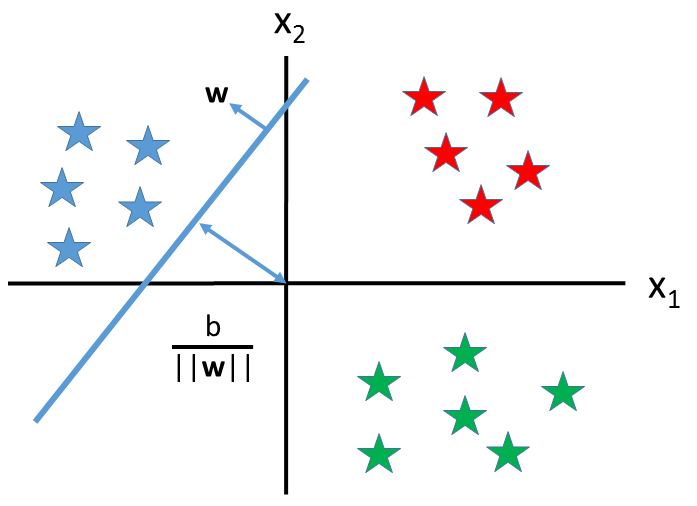
\includegraphics[width=0.65\linewidth]{images/training_set_for_single_layer_hyperplane_v2}
	\caption{One possible dataset describing a three class function. Each class is represented by a different color.}
	\label{fig:training_set_one_layer}
\end{figure}

\subsection{Neural Network Training}

One of the most common methods of training an ANN is through error backpropagation. Error backpropagation is a method to minimizes an error function with respect to the weights connecting neurons as seen in Equation \ref{eq:dMSE}. % If the error function is convex with respect to the network weights, the error with respect to the weights in the network can be minimized using its derivative. THIS IS WRONG. ANN with no hidden layers will have a purely convex error fctn wrt weights, add layers and we get local minima/maxima

Training the simple, one-layer ANN requires finding an expression for \ref{eq:dMSE}. For the following section, let $y_i$ be defined as in Equation \ref{eq:single_layer_eq_sum}, $E_{MSE}$ be defined as the mean squared error function, and training data be defined as in Equation \ref{eq:train_data_D} where $\bold{x_n}$ represents the $n^{th}$ training token and $t_n$ represents the $n^{th}$ binary training target \cite{Nielsen2015}. Note, this derivation would need to be repeated for a different error function. By the chain rule,
%
\begin{equation} \label{eq:dMSE}
\frac{dE_{MSE}}{dw_j} = \frac{dE_{MSE}}{dy_i} \frac{dy_i}{dw_j}.
\end{equation}
%
\begin{equation} \label{eq:train_data_D}
 D={(\boldsymbol{x}_1,t_1), ... ,(\boldsymbol{x}_n,t_n)}
\end{equation}
Equation \ref{eq:dMSE} can be solved by first evaluating $\frac{dE_{MSE}}{dy_i}$,
%
\begin{equation} \label{dE_{MSE}/dy_i}
\frac{dE_{MSE}}{dy_i}  = \frac{d}{dy_i} \sum_i(t_i - y_i)^2
\end{equation}
%
\begin{equation} \label{dE_{MSE}/dy_i}
 = \sum_i  \frac{d}{dy_i} (t_i - y_i)^2
\end{equation}
%
\begin{equation} \label{eq:MSE_deriv}
 =  -2 \sum_i  (t_i - y_i).
\end{equation}
%
Evaluating $\frac{dy_i}{dw_j}$,
%
\begin{equation} \label{dE_{MSE}/dy_i}
\frac{dy_i}{dw_j}  = \frac{d}{dw_j} \tanh( \boldsymbol{w}' \boldsymbol{x}_i + b) 
\end{equation}
%
\begin{equation} \label{dE_{MSE}/dy_i}
 = \tanh'( \boldsymbol{w}' \boldsymbol{x}_i + b) \frac{d}{dw_j}( \boldsymbol{w}' \boldsymbol{x}_i + b)
\end{equation}
%
\begin{equation} \label{dE_{MSE}/dy_i}
 = \tanh'( \boldsymbol{w}' \boldsymbol{x}_i + b)  x_{ij}.
\end{equation}
%
\noindent where $x_{ij}$ is the $j^{th}$ feature of the $i^{th}$ training vector.
%
The update rule for the bias vector is found using
%
\begin{equation} \label{eq:ladidadi}
\frac{dE_{MSE}}{db_j} = \frac{dE_{MSE}}{dy_i} \frac{dy_i}{db_j}.
\end{equation}
%
The expression for $\frac{dE_{MSE}}{dy_i}$ is known from Equation \ref{eq:MSE_deriv}. Evaluating the other derivative in \ref{eq:ladidadi},
%
\begin{equation} \label{dE_{MSE}/dw_j}
\frac{dy_i}{db_j} = \frac{d}{db_j} \tanh(\boldsymbol{w}'\boldsymbol{x}_i + b),
\end{equation}
%
\begin{equation} \label{dE_{MSE}/dy_i}
 = \tanh'( \boldsymbol{w}' \boldsymbol{x}_i + b).
\end{equation}
%
Finally, the gradient of the error function with respect to a single weight can be computed, 
%
\begin{equation} \label{eq:dE_{MSE}/dw_j_final}
\frac{dE_{MSE}}{dw_j} =  -2 \sum_i  (t_i - y_i) \tanh'( \boldsymbol{w}' \boldsymbol{x}_i + b)  x_{ij},
\end{equation}
%
and a single bias,
%
\begin{equation} \label{eq:dE_{MSE}/db_j_final}
\frac{dE_{MSE}}{db_j} =  -2 \sum_i  (t_i - y_i) \tanh'( \boldsymbol{w}' \boldsymbol{x}_i + b).
\end{equation}
%
The derivative in Equations \ref{eq:dE_{MSE}/dw_j_final} and \ref{eq:dE_{MSE}/db_j_final} can used to update each weight and bias in the network as defined by 
%
\begin{equation} \label{eq:update1}
\Delta w_{j} = - \eta \frac{dE_{MSE}}{dw_j}
\end{equation}
%
and 
%
\begin{equation} \label{eq:update2}
\Delta b_{j} = - \eta \frac{dE_{MSE}}{db_j}
\end{equation}
%
where $\eta$ in Equations \ref{eq:update1} and \ref{eq:update2} represents the learning rate of the neural network. The learning rate and its effect on training will be discussed more thoroughly in a later section.

Gradient descent can also be applied to multi-layer ANN. Given an L-layer network where the input stimuli to the $l^{th}$ layer training example x is represented by
%
\begin{equation} \label{eq:CrossEntropy}
\boldsymbol{z}^{x,l} = \boldsymbol{w}^{l}  \boldsymbol{a}^{x,l-1} + \boldsymbol{b}^{l}
\end{equation}
%
where $\boldsymbol{w}^{l}$ is the $l^{th}$ layer's weight matrix, $\boldsymbol{b}^{l}$ is the $l^{th}$ layer's bias vector, and the output activation vector from the $(l-1)^{th}$ layer is 
%
\begin{equation} \label{eq:CrossEntropy}
\boldsymbol{a}^{x,l-1} = f^{l-1}(\boldsymbol{z}^{x,l-1})
\end{equation}
%
where $f^{l-1}$ represents the non-linear activation function used in the $(l-1)^{th}$-layer. Defining the output error as 
%
\begin{equation} \label{eq:CrossEntropy}
\delta^{x,L} = \frac{\partial C}{\partial a^{x,L}} \odot \frac{\partial f^{l-1}(\boldsymbol{z}^{x,l-1}) }{\partial \boldsymbol{z}^{x,l-1}}, 
\end{equation}
%
where $\odot$ is the Hadamard product, the output error can backpropagate to previous layers. For each $l=L-1,L-2,...,2$ an error can be defined by
%
\begin{equation} \label{eq:CrossEntropy}
\delta^{x,l} = ((\boldsymbol{w}^{l+1})^T \delta^{l+1}) \odot \frac{\partial f^{l}(\boldsymbol{z}^{x,l}) }{\partial \boldsymbol{z}^{x,l}}.
\end{equation}
%
The gradient of the cost function as a function of each individual weight and bias can now be defined as 
%
\begin{equation} \label{eq:CrossEntropy1}
\frac{\partial E}{\partial w_{jk}} = a^{l-1}_k \delta^l_j
\end{equation}
%
and 
%
\begin{equation} \label{eq:CrossEntropy2}
\frac{\partial E}{\partial b_j} = \delta^l_j.
\end{equation}
%
Using Equations \ref{eq:update1} and \ref{eq:update2}, the weights can be updated for a single iteration of backpropogation. 

ANNs require some stopping condition to conclude training. One simple stopping condition is ending training when a threshold in network accuracy on a testing set is reached. Where this simple accuracy test is not applicable, such as for regression training sets, a condition based on the ANN training error metric can be used.

Early stopping has the benefit of preventing overfitting and encouraging generalization. Early stopping works by removing a small portion of the training data and defining it as testing data. The ANN is trained using the new training data while some error metric for both the training and testing set are recorded. As training progresses, the ANN likely will overfit to the training data, leading to an increase in error for the testing dataset. Early stopping ends training before overfitting occurs, as illustrated in Figure \ref{fig:training_testing_error}. Because training is stopped before the error in a dataset unknown to the model increases, generalization, or the ability for the ANN to correctly identify patterns outside of the training set, is also improved.

\begin{figure}[H]
	\centering
	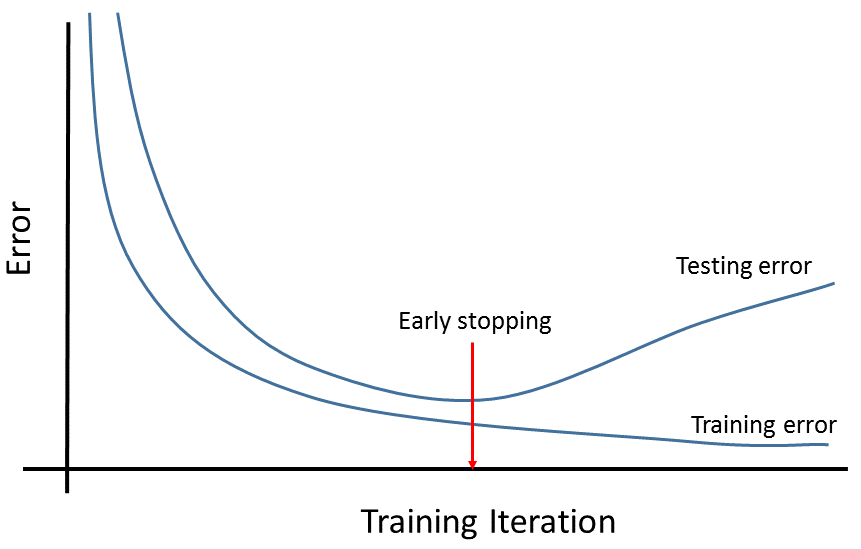
\includegraphics[width=0.85\linewidth]{images/training_testing_error_v2}
	\caption{Ideal training and testing error curves.}
	\label{fig:training_testing_error}
\end{figure}

\subsection{Convolution Neural Networks}

Convolution neural networks (CNNs) use convolutional filters instead of weights. They have been used in image processing. 

One of the first CNN architectures was LeNet-5 \cite{Lecun1998}. LeNet-5 classified 32x32 images of handwritten digits using two convolution-average pooling layers followed by two dense layers and an output. 

AlexNet \cite{Krizhevsky2012} was the first exploration into wider and deeper CNNs. 

Much more work has been done furthering CNNs. VGG \cite{Simonyan2014} showed that smaller filter sizes are good. 

\section{Autoencoders} \label{Autoencoders}
% \cite{CHARTE2018} is a practical guide to autoencoders. Great resource.

Autoencoders were introduced by Hinton \cite{Hinton2006}. They can be used as a method to pre-train networks or as feature extractors \cite{CHARTE2018}.

Other feature extraction methods exist. Principal component analysis (PCA) attempts to reduce the dimensionality of a dataset into linearly uncorrelated variables \cite{Jolliffe2002}. Using a few of these principle components, the data may be represented in a reduced space that contains most of the information present in the original data. Another linear feature extraction method is called linear discriminant analysis (LDA). LDA is a supervised feature extraction method that finds linear combinations of features that can be used to separate classes. Non-linear feature extraction methods, such as kernel PCA, also exist. Kernel PCA applies a non-linear transform to the input space and applies PCA to the data in this transformed space. For kernel PCA to perform well, the correct kernel must be chosen for a given problem, which is a non-trivial task.

Denoising was suggested as a method of extracting useful features from an autoencoder \cite{Vincent2008, Vincent2010}.

\cite{Masci2011} demonstrated that stacking convolution layers made a good autoencoder.

% While autoencoders were touched on in the uranium enrichment work, they have not been explored thoroughly. There is some evidence that the autoencoder was overtrained to the A special case of denoising autoencoders will be explored for the ANSI dataset. 

An autoencoder is an ANN whose goal is to learn a representation of the input. This is accomplished by simultaneously training an encoding ANN and a decoding ANN. An example of this can be seen in Figure \ref{fig:Autoencoder_structure}. As seen in this figure, the encoding ANN reduces an $n-$dimension input signal, $X$, to a $m-$dimension signal, $z$, where $m < n$. The decoding ANN takes the encoded signal, $z$, and outputs a reproduction of the input signal, $X'$.

Without an autoencoder, a single ANN has to learn multiple tasks to identify isotopes. An ANN would have to simultaneously identify the detector calibration, background signal, and possible source signal. By training an autoencoder to reconstruct a background-subtracted and correctly calibrated spectrum, the task of isotope identification is simplified for the ANN. This may result in more accurate identifications. To test this, for each dataset a single autoencoder and three ANNs will be trained. The first will be trained without an autoencoder. The second will be trained using the encoder as input. The third will be trained using the full autoencoder as input. A random hyperparameter search will be used to find an appropriately structured autoencoder. The testing and validation error for these ANNs will be compared for each respective dataset.

% is local spatial structure too much jargon? 
In addition to using fully connected autoencoders, a 1-D convolutional autoencoder will also be explored. A DNN does not assume the input has local spatial structure, while a CNN does. Because gamma-ray spectra have local spatial structure in the form of photopeaks and Compton continua, it may be better to use a CNN over a DNN \cite{CHARTE2018}. To test this, the experiment described above will be repeated using a 1-D convolutional autoencoder.

% Or I might just use the 1D convolutional autoencoder because it makes more sense

\begin{figure}[H]
\centering
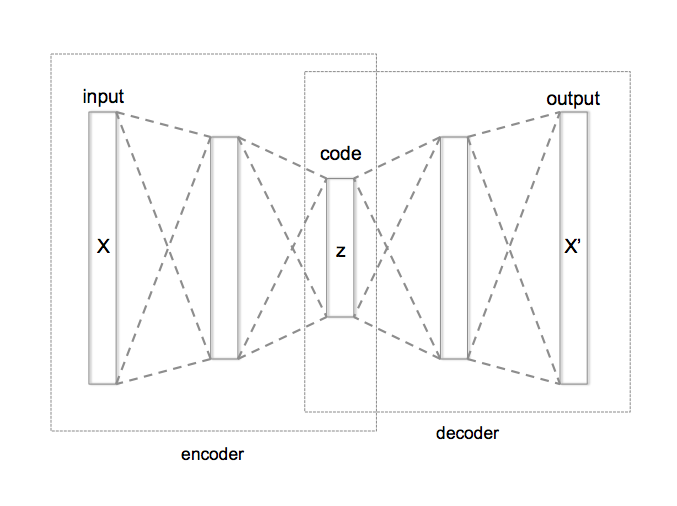
\includegraphics[width=0.8\linewidth]{images/Autoencoder_structure}
\caption{An example of an autoencoder \cite{wiki:AutoencoderStructure}.}
\label{fig:Autoencoder_structure}
\end{figure}


% Fully connected ANNs do not assume there is local spatial structure in a signal, so the fully connected ANN would need to learn that there is local structure. Convolutional ANNs assume there is local structure, and the extent of this structure can be changed by changing the length of the convolutional ANNs filters.

% Once the autoencoder is trained, the hidden layer and output layer (representing the reconstructed spectrum) will be used to train a separate ANN for isotope identification and quantification. The performance of these ANNs will be compared.



\subsection{Hyperparameters}

In addition to the weights connecting neurons, ANNs can have additional hyperparameters. Hyperparameters determine both the networks structure (number of layers, number of nodes in each layer, activation function for each layer) and how the model learns (learning rate, momentum, loss function). In the following section, various hyperparameters and their effects on ANN learning are discussed.

\subsubsection{Learning Rate}

The learning rate is a tunable parameter that affects the magnitude of each weight update. If $\eta$ is too small, the network will learn slowly and training will be inefficient. If $\eta$ is too large, the network will fail to learn, either by converging to a non-extremum or by diverging. An example of a small and large learning rate are shown in Figure \ref{fig:Learning_rate_comparison} 

\begin{figure}[H]
	\centering
	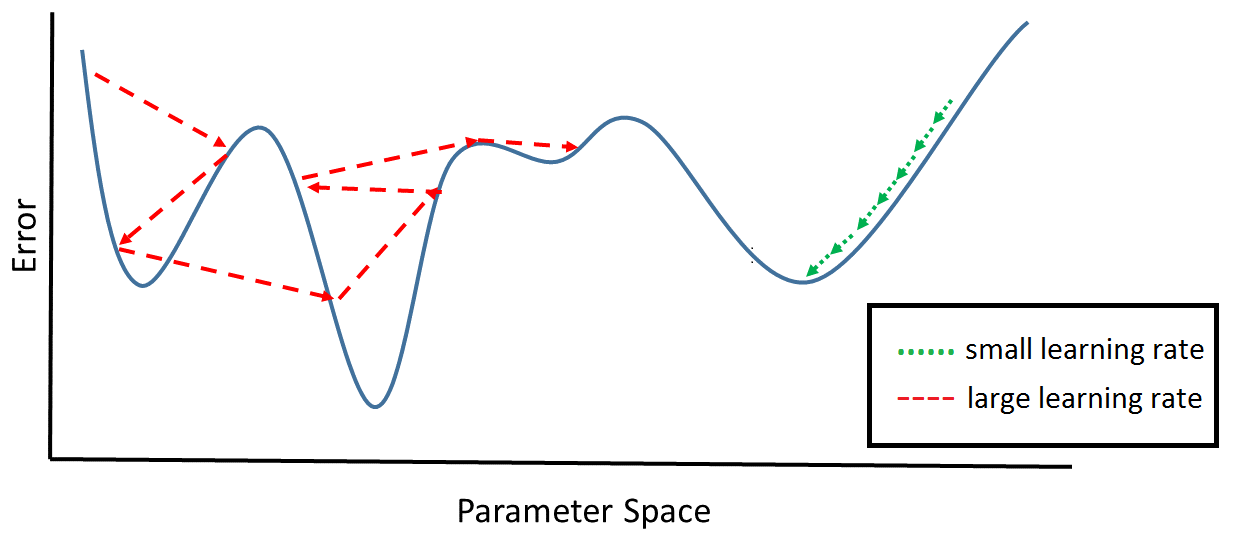
\includegraphics[width=0.8\linewidth]{images/Learning_rate_comparison_v2}
	\caption{Example training paths for a large learning rate, red, and a small learning rate, green.}
	\label{fig:Learning_rate_comparison}
\end{figure}


There are many methods to modify $\eta$ to encourage more efficient learning. One method to increase the speed of learning is to start with a large $\eta$ and decrease $\eta$ as a function of iteration number. Ideally, this method would lead to quick initial learning when far from an optima and slower learning near an optima to more finely explore it. The difficulty with this method is the requirement for a function that slows the learning rate efficiently for a given problem.

\subsubsection{Learning Momentum}

Another method to speed up learning is to add a momentum hyperparameter, $\mu$, to the weight update algorithm \cite{Yu1997}, 
%
\begin{equation} \label{eq:update_momentum}
\Delta w_{ij}(n) = - \eta \frac{dE_{MSE}}{dw_j} +\mu \Delta w_{ij}(n-1).
\end{equation}
%
Similar to the goal of slowing learning over time described above, the momentum term attempts to slow learning near optima. The momentum will be large when the weights are updated at large steps, far from an optima, but will decrease near an optima, allowing slower learning near an optimum.
 
\subsubsection{Training Algorithms}

There are many ANN training algorithms that employ clever learning rate schedules and momentum functions. These algorithms include but are not limited to: Nesterov's accelerated gradient \cite{nesterov1983}, simulated annealing \cite{Kirkpatrick1983}, ADADELTA \cite{ADADELTA}, and ADAM \cite{Kingma2015}. 

The ADAM optimizer was chosen as the training algorithm for the work presented in this thesis due to its incorporation of parts of other successful optimization algorithms and its reported superior performance over these algorithms. Another benefit of the ADAM optimizer is introduction of only one hyperparameter, the learning rate. 

The ADAM optimizer update rule is described below. For the following, $g_t$ is the gradient of the error function with respect to the network parameters at iteration $t$, 
\begin{equation} \label{eq:adam1}
m_t = \beta_1 m_{t-1} + (1 - \beta_1) g_t,
\end{equation}
is the estimate of the mean of the gradient at iteration $t$ and
\begin{equation} \label{eq:adam2}
v_t = \beta_2 v_{t-1} + (1 - \beta_2) g_t^2
\end{equation}
is the estimate of the variance of the gradient at iteration $t$. For the following, the variables $\beta_1$ and $\beta_2$ are parameters called decay rates, $\epsilon$ is another parameter, and $\theta_t$ represents the network parameters at iteration $t$. As described by Kingma and Lei Ba, The default values for $\beta_1$, $\beta_2$, and $\epsilon$ are 0.9, 0.999, and $10^{-8}$ respectively \cite{Kingma2015}. These values were seen to work well for a variety of problems. While these hyperparameters can also be tuned, it has been shown that the default values work well for a variety of network architectures and datasets \cite{Kingma2015}. The bias-corrected first moment estimate is given by
\begin{equation} \label{eq:adam3}
\hat{m}_t = \dfrac{m_t}{1 - \beta^t_1}
\end{equation}
and the bias-corrected second moment estimate is given by 
\begin{equation} \label{eq:adam4}
\hat{v}_t = \dfrac{v_t}{1 - \beta^t_2}.
\end{equation}
Finally, the weight update equation is computed as
\begin{equation} \label{eq:adam5}
\theta_{t+1} = \theta_{t} - \dfrac{\eta}{\sqrt{\hat{v}_t} + \epsilon} \hat{m}_t.
\end{equation}


%Due to the number of free parameters in a ANN (each hidden layer weight is a free parameter), these models have a tendency to overfit data. The three methods used to prevent overfitting in this thesis are $L_2$ regularization, neuron dropout, and data augmentation. These techniques greatly improve the performance of the presented ANN. 

% Is this neccesary? Just mentioning it is enough I think.

%Another method is to randomly perturbing the weights during training using a simulated annealing technique \cite{Kirkpatrick1983}. Simulated annealing mimics how crystal lattices bond together in cooling metal to achieve a low energy state. As metal cools, its crystal lattice will orient itself to lower its total bond energy, but occasionally due to statistical heating sections will jump to a higher energy level. This encourages a global low energy state, as many local low energy state regions are discouraged. This process can be mimicked in a learning algorithm by randomly perturbing the weights during learning. As learning continues the network 'cools' and the frequency of weight perturbation decreases. It can be shown that given a long enough annealing schedule, the global optimum solution for a problem is guaranteed to be found \cite{Granville1994}.

\subsubsection{Cost Function}

The choice of cost function to train against depends on the targets the network is attempting to learn. One of the simplest error functions is the binary accuracy for classification, 
%
\begin{equation} \label{eq:Binary_accuracy}
E_{Binary} = {\frac{1} N} \sum_{n=1}^N [\hat{y}_n \neq y_n ],
\end{equation}
%
where N is the total number of output neurons, $y_n$ is the ground truth of the n$^{th}$ output, and $\hat{y}_n$ is the ANN output of the n$^{th}$ output neuron. While this is a simple function, it penalizes the model for being close to the answer. Because there is no incremental indication that a model is improving, this error function is not typically used for gradient descent algorithms.

A simple differentiable cost function is the mean squared error (MSE) function shown in Equation \ref{eq:MSE_error}. This function is differentiable, so gradient descent algorithms can be applied to it. The MSE function is appropriate when targets are any real number, as in a regression problem. 
%
\begin{equation} \label{eq:MSE_error}
E_{Binary} = {\frac{1} N} \sum_{n=1}^N (\hat{y}_n - y_n)^2,
\end{equation}
%
For classification problems, the average cross entropy, shown in Equation \ref{eq:CrossEntropy} can be used. Cross entropy measures how different the probability distributions $y_n$ and $\hat{y}_n$ are from each other. Because the cross entropy treats $y_n$ and $\hat{y}_n$ as probability distributions, they are required to exist in the range [0,1].
%
\begin{equation} \label{eq:CrossEntropy}
E = -{\frac{1} N} \sum_{n=1}^N y_n \log(\hat{y}_n) +  (1-y_n) \log(1-\hat{y}_n), 
\end{equation}
%

Because the softmax function can be used for classification, it is traditionally used as the output function for the model when using the cross entropy cost function. The softmax function is used in binary classification problems to calculate posterior class probabilities \cite{Bridle1990}.

\begin{equation} \label{eq:softmax}
softmax(z_j) = \frac{\exp(z_j)} {\sum_{k=1}^{K} \exp(z_k)}.
\end{equation}


%% This part is kinda total butts
%It is important to note that for a single layer neural network with the MSE cost function, the one minimum in $MSE(W)$ is the global minimum. When the number of layers increases beyond one there may be many more local minima in the cost function. Care must be taken when training a neural network to either find the global minimum in the cost function with respect to the weights or to find a minimum that reduces the error below a desired value. Care must also be taken to avoid stuck training, or having the optimization algorithm find a local minimum and not move from it. A proper optimization technique must account for these pitfalls. 

\subsubsection{Weight Regularization}

Weight regularization is a hyperparameter that penalizes the ANN when the magnitude of the weights increases. Because the magnitude of the weights is tied to the complexity of the model, adding weight regularization attempts to limit complexity and the probability of overfitting.

A common method of incorporating weight regularization is by adding an $L_n$ regularization term to the error function, as seen in Equation \ref{eq:L2_Reg}. Common values for $n$ are 1 and 2. Adding weight regularization allows the magnitude of the weights to increase only when there is a comparable reduction in the unmodified error function.
%
\begin{equation} \label{eq:L2_Reg}
\tilde{E} = E + \sum_i \lambda w_i^n.
\end{equation}
%
In Equation \ref{eq:L2_Reg}, $w_i$ is the weight between each neuron in the ANN and $\lambda$ is the regularization strength hyperparameter. A larger $\lambda$ will force the ANN to prefer smaller weights connecting the neurons. If the parameter $\lambda$ is too small, the unbounded model complexity may fit only the training data. If the parameter $\lambda$ is too large, the ANN will only minimize the $L_n$ error, failing to learn.

\subsubsection{Neuron Dropout}

Another method to reduce model complexity is neuron dropout. Neuron dropout is the process of temporarily removing a neuron from the ANN architecture \cite{Srivastava2014}. By randomly removing neurons from an ANN during training, heavy local codependency between neurons that could lead to the ANN becoming stuck in a local minimum in the error function, and thus overtraining, is discouraged. The frequency with which neurons are removed is called the neuron dropout rate, which is a hyperparameter.

Almost always, taking the average output of more than one separately trained ANN improves the performance of the ANN \cite{Srivastava2014}. By applying dropout at each neuron with the same probability throughout training, the ANN's architecture changes every iteration. The makes neuron dropout a cost efficient way to effectively average many different ANN architectures, improving performance.

\subsubsection{Data Augmentation}

Data augmentation changes the data during training using physically realistic transformations. For example, a training dataset of images can be rotated, flipped, blurred, or color augmented during training. An example of horizontal flip and a blur augmentation are seen in Figure \ref{fig:cat}. This cheaply expands the training dataset and discourages overtraining, as the ANN never observes the exact same image. Both the augmentation method and strength of said method are hyperparameters. 

\begin{figure}[H]
	\centering
	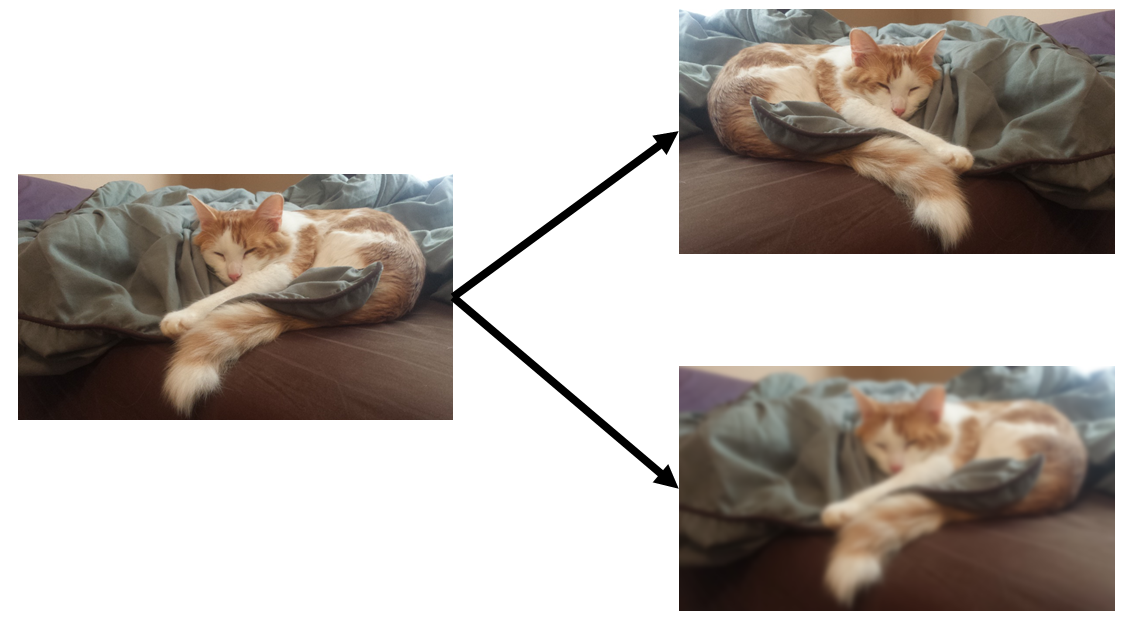
\includegraphics[width=0.9\linewidth]{images/cat}
	\caption{Two examples of data augmentation using an image of a cat. The image to the left is the original. The top right image is augmented using a horizontal flip. The bottom right image is augmented using blur.}
	\label{fig:cat}
\end{figure}

\subsection{Hyperparameter Optimization}

In general, ANNs have many hyperparameters that require optimization. Optimizing these hyperparameters will lead to more efficient training and more accurate performance when training is concluded. There are several different methods to perform hyperparameter optimization for an ANN. These methods may include manual optimization, exhaustive grid search, and random parameter search.

Manually optimizing parameters is necessary when developing a novel algorithm. This involves changing hyperparameters and observing how the ANN trains and the final error on a validation dataset. Ideally, the ANN should train quickly and have a low error on a validation dataset. For many parameters `rule of thumb' values exist that can be used to find parameters that work to some degree. Due to the large hyperparameter space, a manual search is cost prohibitive if further optimization is desired.

Once a range of parameters is determined through a manual search, multiple methods are available to explore the parameter space for an optimal solution. One method is an exhaustive grid search. In a grid search the parameter space is divided into a uniform grid and the joint performance of all parameters is tested. The grid search method is ineffective for two reasons. First, neural networks may have a large number of hyperparameters that need to be explored, and the computational requirement to explore the hyperparameter space increases exponentially with increasing hyperparamters. Second, in practice only a few hyperparameters dominate performance, but the dominating hyperparameters are different for different applications. A grid search may under represent the importance of key hyperparamters, as seen in Figure \ref{fig:Bergstra12a_hyperparameter_grid_vs_random}.  While this method works, it has been shown that a random search in the hyperparameter target domain finds better hyperparameters quicker than testing equally distributed points in the chosen range \cite{Bergstra2012}. It can also be shown that given 60 random samples over some space with a finite minimum, the minimum of those 60 random samples is within 5\% of the true minimum with 95\% probability \cite{Zheng2015}. This means that given a range of hyperparameters, the best performing hyperparameter combination out of 60 randomly sampled points is very likely to be close to optimal. 

\begin{figure}[H]
	\centering
	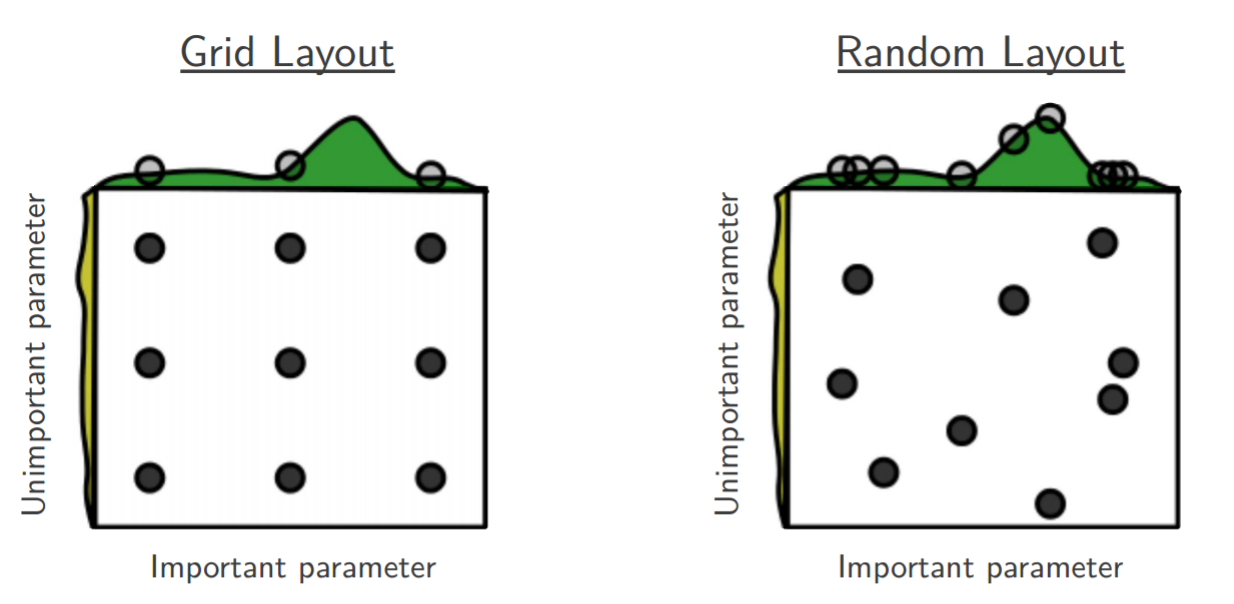
\includegraphics[width=0.99\linewidth]{images/Bergstra12a_hyperparameter_grid_vs_random}
	\caption{A comparison between a grid search and a random search for hyperparameter optimization when performance is strongly tied to one hyperparameter. The green function represents the effect of an important hyperparameter on a cost function while the yellow function represents the effect for an unimportant hyperparameter. Figure reproduced from [42].}
	\label{fig:Bergstra12a_hyperparameter_grid_vs_random}
\end{figure}


The ability for an ANN to solve a problem depends on the network structure, teaching method, and the training set to be learned. In the following section, a method for generating a training set for isotope identification and quantification is described.

To analyze the performance of a random search, a random hyperparameter efficiency curve, example shown in Figure \ref{fig:Bergstra_random_efficiency_curve_DNN} can be used. In the figure, 256 hyperparameter searches are run. These trials are split into experiments with sizes of increasing powers of two. The best performing trial from each experiment is determined and shown using a box plot.


\begin{figure}[H]
	\centering
	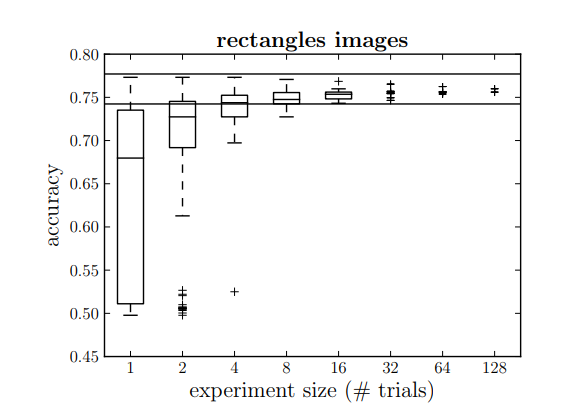
\includegraphics[width=0.9\linewidth]{model_choice_hyperparameter_search_images/Bergstra12_random_efficiency_curve}
	\caption{Example Random efficiency curves for a neural network \cite{Bergstra2012}.}
	\label{fig:Bergstra_random_efficiency_curve_DNN}
\end{figure}



\section{Summary}

In this chapter, the structure of multi-layer ANNs, methods to train and optimize them, and a method to create a training set for isotope identification and quantification have been described. In the following section an ANN will be presented using these concepts and its performance on a number of real and simulated spectra will be discussed. 










